\usetikzlibrary{graphs, shapes.geometric, positioning}% Enable the shadings library
\usetikzlibrary{shadings}
\usetikzlibrary {arrows.meta}
\definecolor{vibrantblue}{HTML}{48bfe3}

\begin{frame}
    \frametitle{What is PLM?}
    \begin{center}
        % Main title "PLM"
        \begin{tikzpicture}[remember picture,overlay,node distance=.1mm]
            % Title text
            \node[rectangle,fill=white](org) at (0,0){};
            \node[rectangle, rounded corners, shading=axis, top color=blue!50, bottom color=cyan!20,, align=center, minimum width=10cm,drop shadow, above=1cm of org]
            {A Protein Language Model is a language model\\ that applies the principles of natural language processing \\to predict how proteins fold and function};

            \pause
            \node[circle,left=1.7cm of org, yshift=-1.9cm,,circular glow,outer color=blue!30,inner color=white,, inner sep=0pt](seq){ 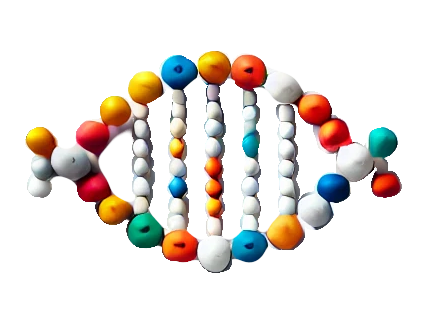
\includegraphics[width = 3.2cm]{images/sequence.png}};
            \pause
            \node[circle,right=1.7cm of org, yshift=-2cm,circular glow,outer color=purple!30,inner color=white,, inner sep=0pt](struct){ 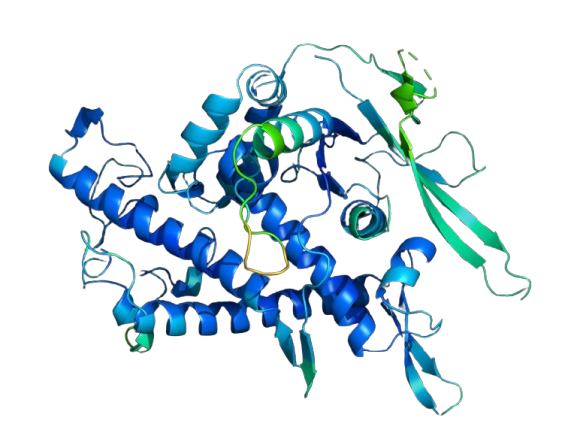
\includegraphics[width = 3.2cm]{images/structprot2.png}};
            \pause
            \node[below=.05cm of org,draw, shading=axis, left color=blue!30, right color=purple!30, text centered, rounded corners, minimum height=3.5cm, minimum width=1.8cm](plm){\textbf{PLM}};

            \draw [red, arrows = {-Stealth[color=blue]}] (seq) to [yshift=-15pt](plm);
             \draw[red, arrows = {-Stealth[color=blue]}] (plm) to [yshift=10pt](struct);

            % % Subtitles with matching colored initials
            % \node[font=\large\bfseries, text=black] at (0, 0.5) {\textcolor{darkblue}{P}ROTEIN};
            % \node[font=\large\bfseries, text=black] at (0, -0.5) {\textcolor{darkblue}{L}ANGUAGE};
            % \node[font=\large\bfseries, text=black] at (0, -1.5) {\textcolor{darkblue}{M}ODEL};
        \end{tikzpicture}
    \end{center}
\end{frame}
